\documentclass{article}

% Language setting
% Replace `english' with e.g. `spanish' to change the document language
\usepackage[english]{babel}

% Set page size and margins
% Replace `letterpaper' with`a4paper' for UK/EU standard size
\usepackage[letterpaper,top=2cm,bottom=2cm,left=3cm,right=3cm,marginparwidth=1.75cm]{geometry}

% Useful packages
\usepackage{amsmath}
\usepackage{graphicx}
\usepackage[colorlinks=true, allcolors=blue]{hyperref}

\title{CPE301L: Lab 1}
\author{Joshua Knight, Nicky Victoriano}

\begin{document}
\maketitle

\section{Introduction}

In this lab, we are responsible for programming an Arduino to respond to a button press. Upon pressing the button, there will be a light that activates and a message in the Arduino IDE's serial monitor signaling that the button is being pressed. When the button is unpressed, the light will be off and there will be no message. This task involves both reading in data and outputting data.

\section{Questions}

\subsection{What is a pin on the Arduino?}

A pin on an Arduino is a register that serves as an input or output.

\subsection{What is the Serial port in reference to the Arduino ATMega 2560?}

The serial port is the digital signal that lets the Arduino communicate to the computer over USB. In the lab, the serial port was communicating with the computer using Universal Serial Bus (USB).

\subsection{How is analog data different from digital data?}

Analog data are a continuous set of data that can represent values in between two points (such as decimal values). Meanwhile, digital is discrete and communicated in whole values (like 0 and 1).

\section{Results}

\subsection{Circuit}

To create our circuit \textbf{Figure \ref{fig:circuit-off}}, we set up the ground and power connections between the appropriate rails. Once this was set up, we connected a button with pull-down resistor to the ground and a connection to pin 2 of the Arduino to send input signals. Then, we used pin 4 of the Arduino and connected it to an LED to act as an output signal. Finally, we connected the serial port of our Arduino to the computer so that the program can run and the serial monitor can also receive the output signal. The final outcome can be seen in \textbf{Figure \ref{fig:circuit-on}}, 

\begin{figure}
\centering
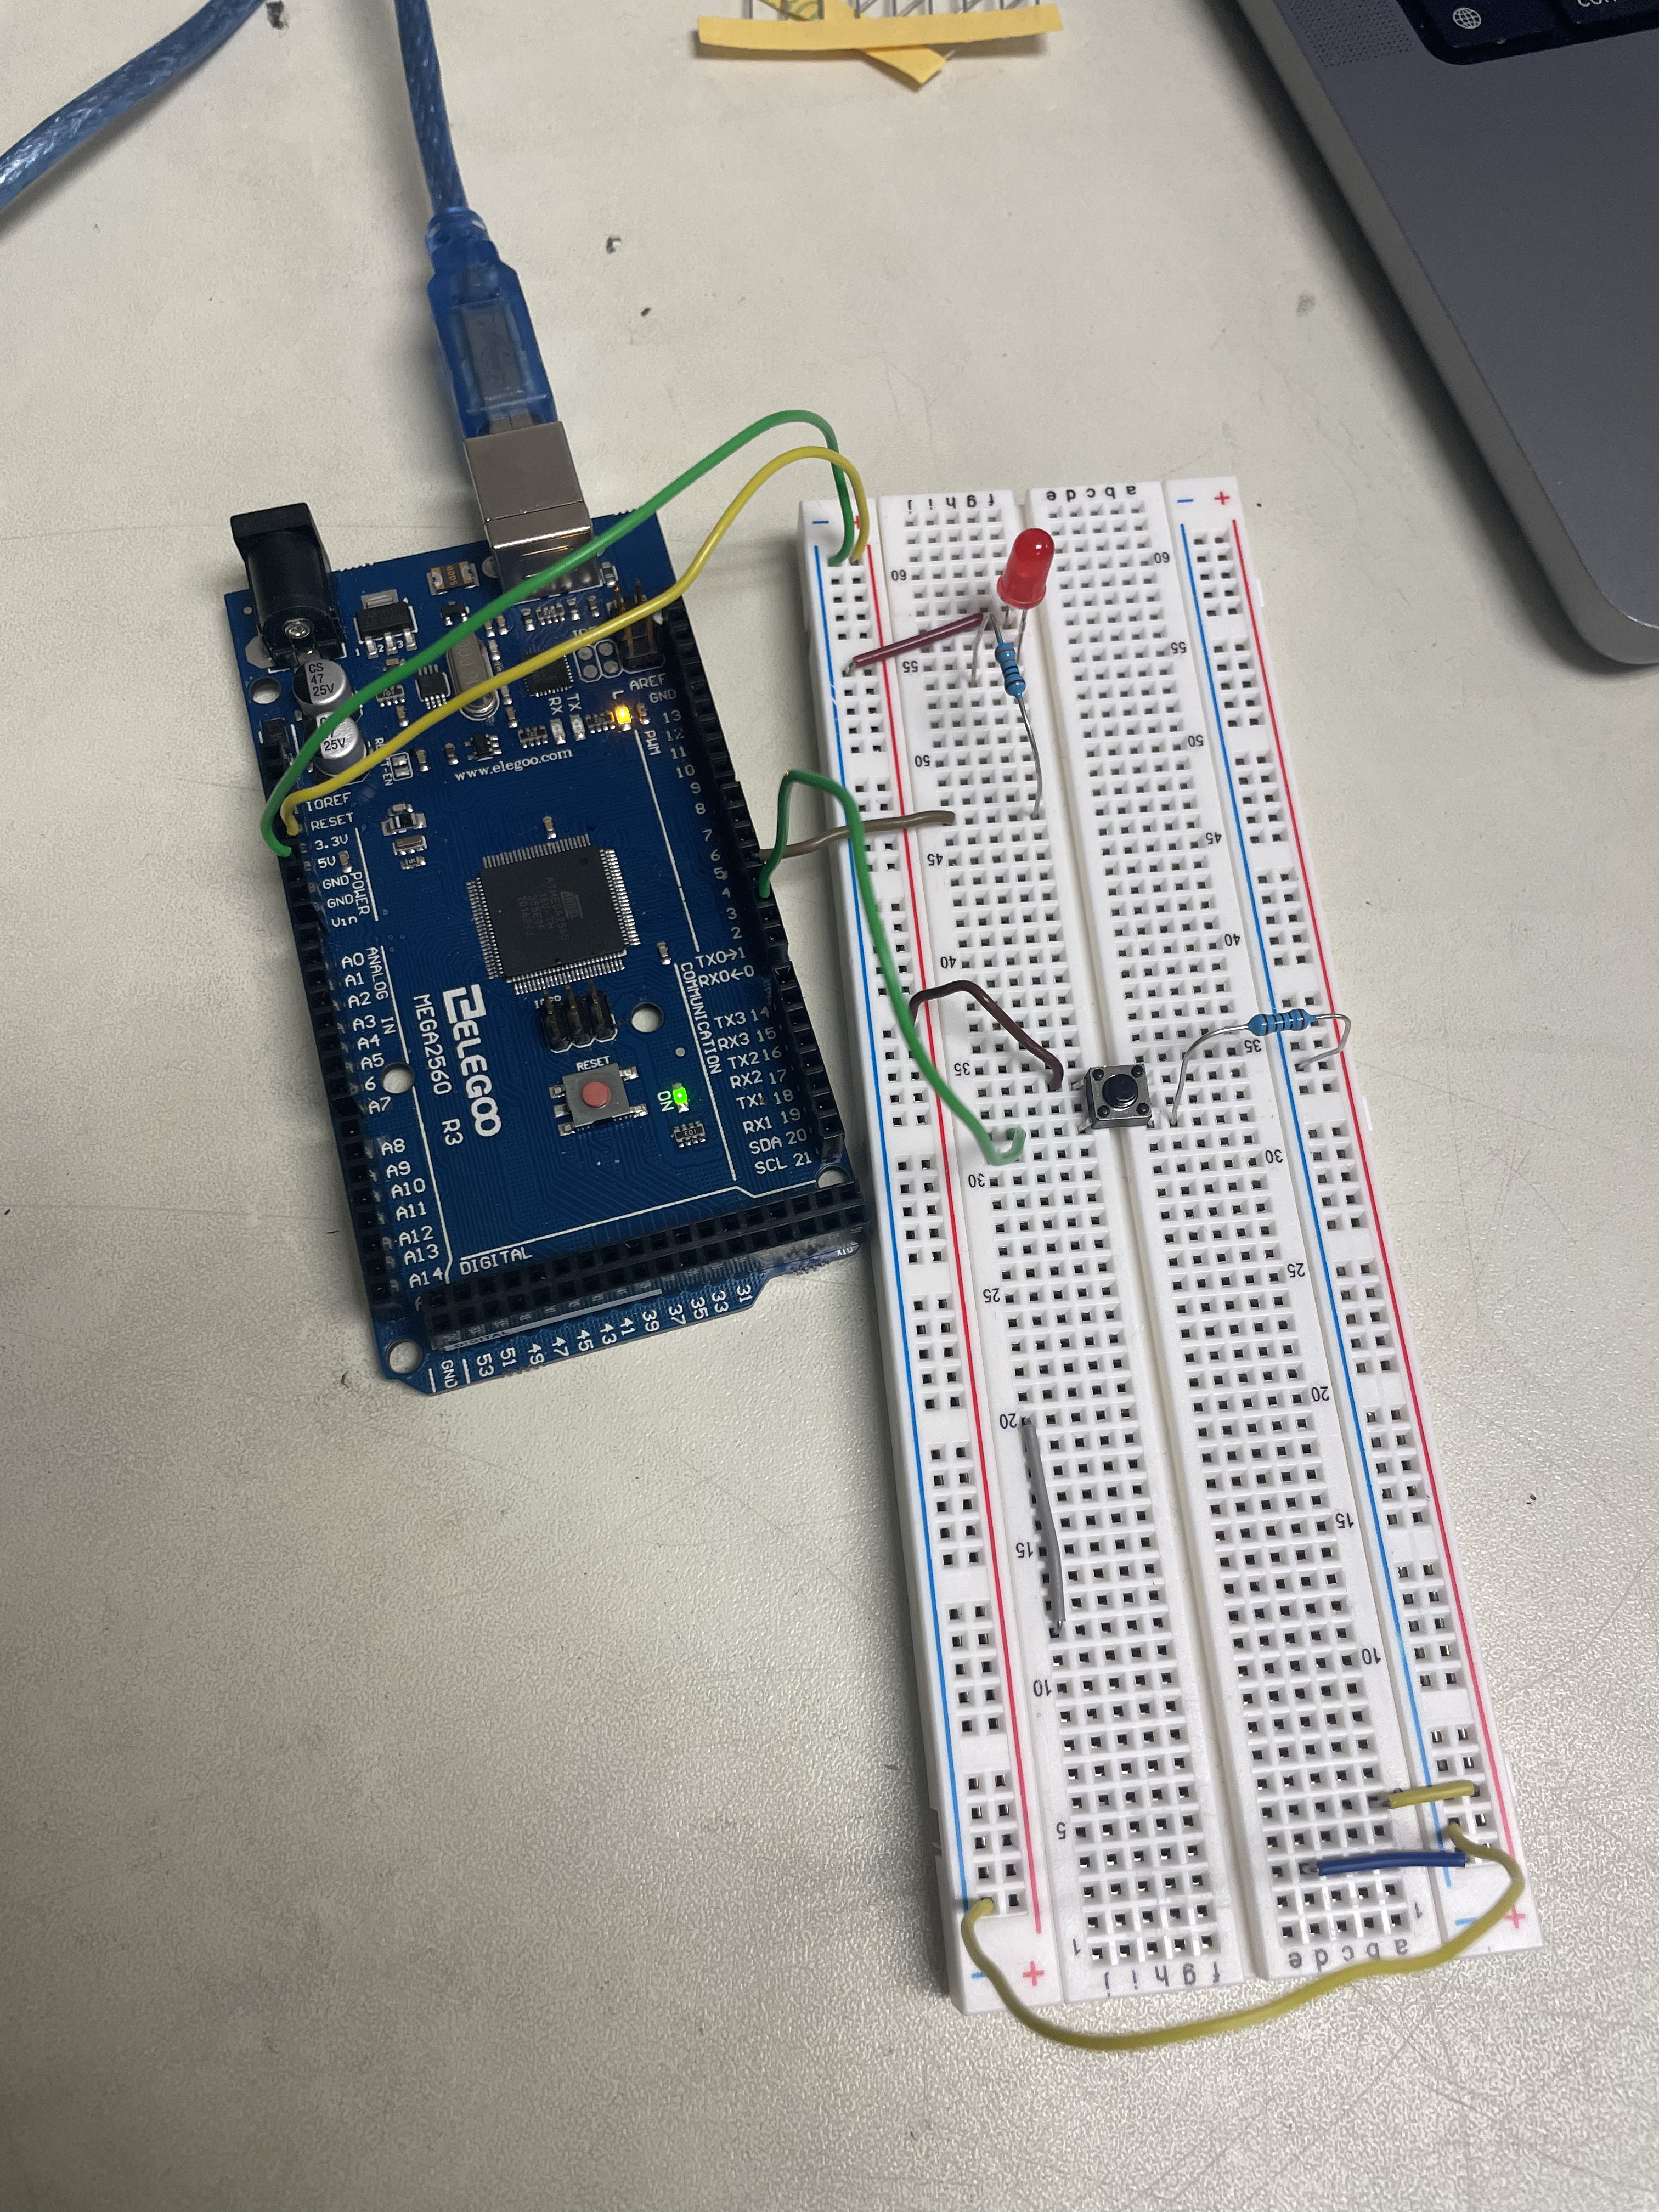
\includegraphics[width=0.5\textwidth]{circuit-off.jpg}
\caption{\label{fig:circuit-off}This is the full circuit created.}
\end{figure}

\begin{figure}
\centering
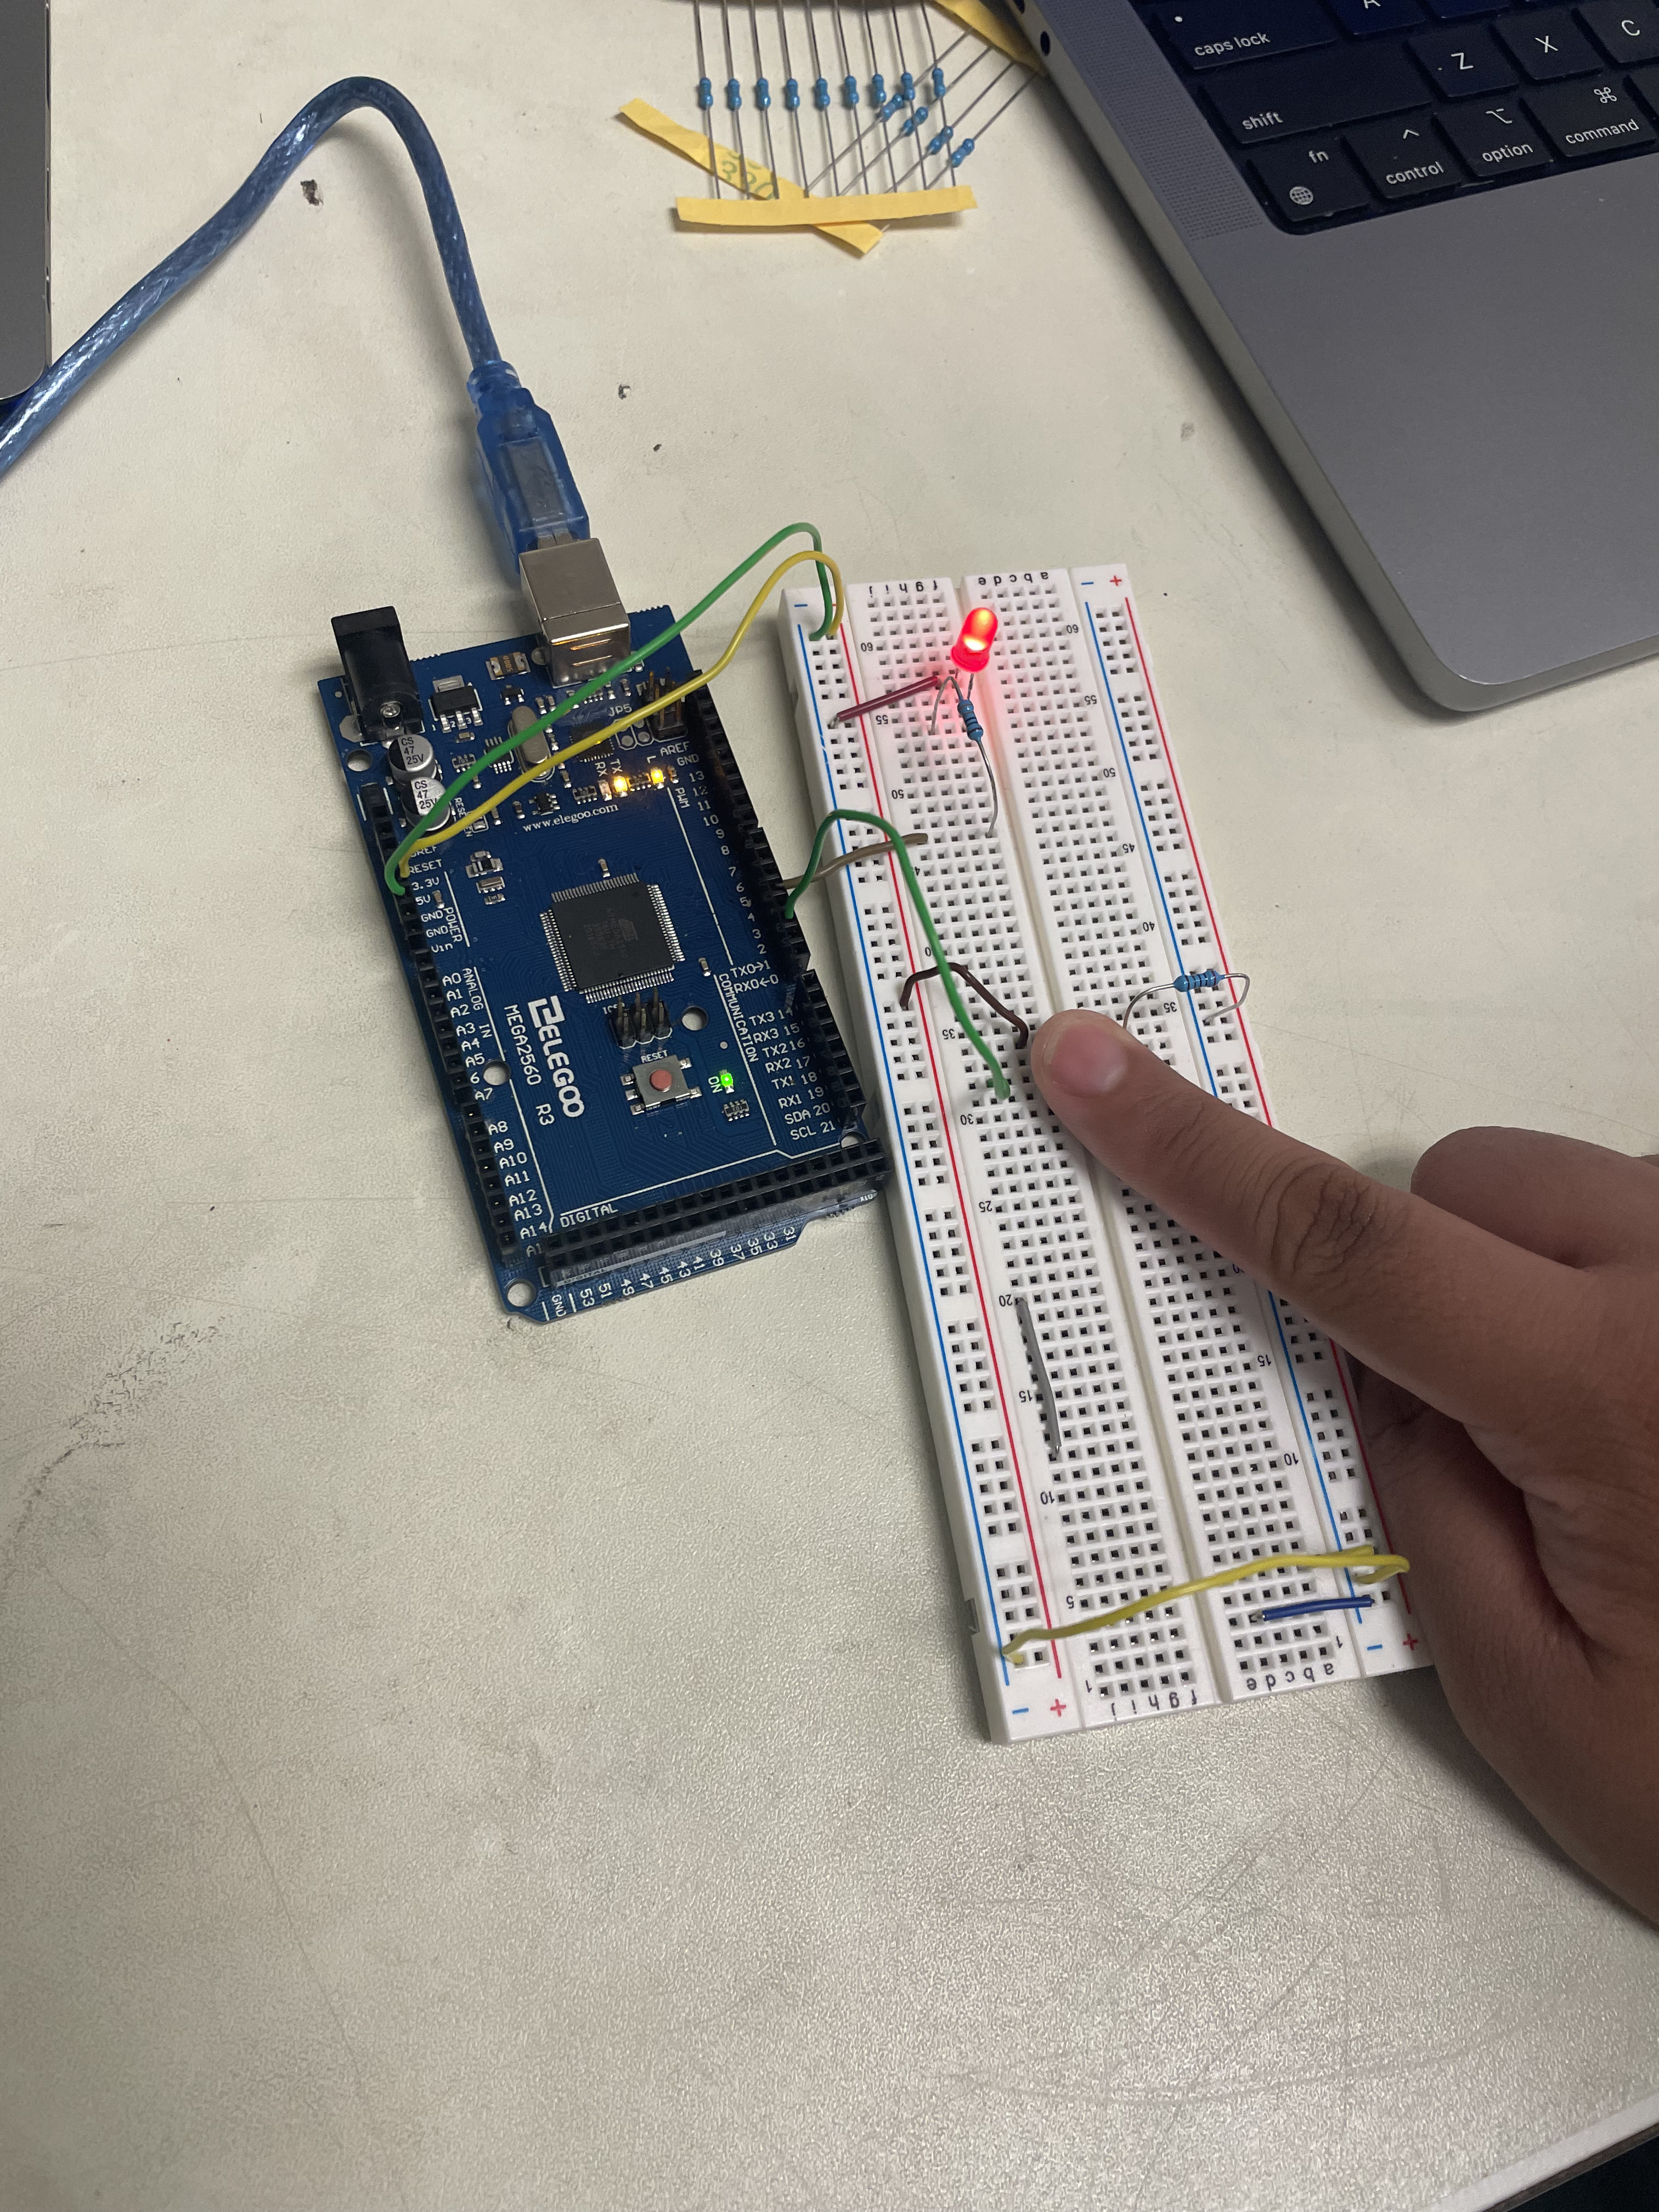
\includegraphics[width=0.5\textwidth]{circuit-on.jpg}
\caption{\label{fig:circuit-on}This is the circuit working on proof.}
\end{figure}

\subsection{Code}

The code was made on Arduino IDE, heavily based on the code included in the lecture slides. The code initializes the serial connection to the computer, before going into it's main loop. In the main loop, the arduino checks for a digital signal on pin 2. If the signal reads 'HIGH' a "button press" message is logged to the serial port and the LED flashes for a moment. Otherwise, the LED output pin is set to 'LOW' (off).

View code on \href{GitHub}{https://github.com/jrkre/cpe-301}.


\end{document}